\documentclass[8pt, a4paper]{article} % Класс документа: статья, шрифт 8pt, формат бумаги A4
\usepackage{hyperref} % Для добавления гиперссылок
\usepackage[utf8]{inputenc} % Кодировка UTF-8 для поддержки специальных символов
\usepackage{multicol} % Для использования нескольких колонок в тексте
\usepackage{setspace} % Для настройки межстрочного интервала
\usepackage{ragged2e} % Для выравнивания текста по ширине
\usepackage{fancyhdr} % Для настройки верхних и нижних колонтитулов
\usepackage{titlesec} % Для настройки стилей заголовков
\usepackage{graphicx} % Для вставки изображений
\usepackage{float} % Для точного управления положением "плавающих" объектов (картинок, таблиц и т. д.)
\usepackage{wrapfig} % Для обтекания текста вокруг фигур (картинок, таблиц и т. д.)


\usepackage[left=1.9cm,right=1.9cm, top=2.2cm,bottom=2cm]{geometry}

\justifying % выравнивает текст по ширине.
\fancyhf{} %очищает все верхние и нижние колонтитулы.

\renewcommand{\headrulewidth}{0pt} % remove the header rule
\cfoot{\vskip -1.5cm \thepage} %устанавливает номер страницы в нижнем колонтитуле.

\linespread{0.81} %устанавливает межстрочный интервал в 0.81
\setlength{\columnsep}{0.5cm}
\setcounter{page} {190}
\renewcommand{\thesection}{\Roman{section}}
\setcounter{section}{1}
%устанавливает стиль нумерации разделов в виде заглавных римских цифр.

\titleformat{\section}{\footnotesize\centering\sc\bfseries}{\thesection.}{0cm}{}[] %настраивает стиль заголовков разделов.

\begin{document}


\fontsize{80}{14}\selectfont
\begin{multicols}{2}
\setlength{\parindent}{0.8cm}
\setlength{\parindent}{0.4cm}
\fontsize{10}{15}\selectfont 
 
 \quad And software tools for building geological models of soil layers, multi-layer reservoirs; the Generator of the geological model of a deposit (GGMD)the integrated software complex of the composer of digital geological and geoecological models.

\fontsize{10}{14}\selectfont
\quad Wenote the main additions to the GeoBazaDannych,
including methodological aspects and software components implemented using artificial intelligence tools. At
the same time, in order to understand the stages of
development and the relationship of the components, we
will give examples of the use of updated components of
the complex and recall fragments of the results that were discussed and published in the proceedings of OSTIS.

\fontsize{10}{14}\selectfont
\quad We note the main additions to the GeoBazaDannych, including methodological aspects and software components implemented using artificial intelligence tools. At
the same time, in order to understand the stages of
development and the relationship of the components, we
will give examples of the use of updated components of
the complex and recall fragments of the results that were discussed and published in the proceedings of OSTIS.

\fontsize{10}{14}\selectfont
\quad In recent years, the activity of using artificial intelligence tools in solving problems of geology and geoecology has been rapidly increasing. In particular, dozens of articles are published every year on the algorithms and methods of cluster analysis considered in this paper. There are publications that provide solutions to practical
problems, methods of preprocessing and interpretation
of geophysical data, anal of conclusions and recommendations (for example, [5], [6]).

\fontsize{10}{14}\selectfont
\quad A number of features of data preparation for computer based geological and geoecological models from the perspective of the feasibility of using artificial intelligence tools have been regularly discussed at OSTIS conferences since 2019. We will note only the typical difficulties that arise when developing tools and conducting computational experiments for specific practical tasks, which
were identified and solutions are presented in subsequent
results

\fontsize{10}{14}
\selectfont
\quad Thus, in the materials of the OSTIS-2019 conference (“Examples of the use of artificial neural networks in the analysis of geodata"), methodological and technical solutions, software tools, results and examples of data processing typical for geophysical methods of studying geological objects, in particular, on observation profiles, were discussed and published. The effectiveness of the use of artificial neural networks to eliminate noise and
errors in the measurement results, perform the necessary data preprocessing for mathematical models by smoothing in order to prepare regular digital distributions is illustrated.

\fontsize{10}{14}
\selectfont
\quad In the materials of the OSTIS-2020 conference (“Examples of intelligent adaptation of digital fields by means of the GeoBazaDannych system“ and ”Interactive Adaptation of Digital Fields in the GeoBazaDannych System"), examples of interactive formation of digital models of geological and geoecological objects in computational experiments that meet the intuitive requirements of an expert are considered and given. Methodological and algorithmic solutions effective in processing remote environmental monitoring data, special tools of the GeoBazaDannych system are noted, the results of interactive adaptation and comparison with standard reference solutions in the complex "Generator of the geological model of the deposit" are resented.

\fontsize{10}{14}
\selectfont
\quad The examples show that this way you can significantly improve the quality and adequacy of the digital description. But you need to understand that at that stage of the state of the algorithmic and software complex of GeoBazaDannych, the allocation itself is implemented according to the intuitive suggestions of the expert.

\fontsize{10}{14}
\selectfont
\quad The issues of automatic identification of sites of the “highlighted” type using cluster analysis tools integrated into the GeoBazaDannych system were discussed at the OSTIS-2022 conference; some positive results were published in the proceedings of the conference and in [7]. In particular, the results illustrating the effects of choosing and confirming the best clustering algorithms are presented, and the options for using different clustering methods are compared, moreover, for different ways of setting the metric distance. In the above-mentioned published materials of OSTIS-2022, along with the positive ones, the disadvantages of the described software
implementations and the settings used were noted.

\fontsize{10}{14}
\selectfont 
\quad
A number of additions to the GeoBazaDannych complex, other variations of the settings of the Wolfram
Mathematica system tools for data clustering have been
tested in calculations, visualized and described below. Nevertheless, it should be understood that further research, improvement of algorithms and modification of software tools are needed.

\fontsize{10}{15}
\selectfont
 \section{\textbf{Initial data, a reference distribution for computational experiments}}

 
\fontsize{10}{14}
\selectfont 
\quad
The results below cannot be strictly mathematically
justified, but are indicative and adequate due to the rules of their preparation. On the one hand, they are being formed by random number generators and refined by an expert in order to give them the character of comparable data from field observations in the practice of geophysical methods for studying geological, geoecological objects On the other hand, accepted mathematical expressions are used for measurement values in observations (in calculations, this is an imitation). In fact, for each particular processing algorithm, it is known that the basic
(reference) digital distribution can be calculated with the necessary accuracy — comparing calculations with the standard, one can judge the advantages and disadvantages of the method used. Below, the reference distribution (in the accepted GeoBazaDannych terminology, the surface)
differs slightly from that considered in [4], the location of the fragments of disturbances and their shape and dimensions have been changed for some. Generally speaking, there was no need for changes, because the set of fragments of typical relief elements in [4] was quite representative, but calculations were performed specifically for a reference surface of a different shape to ensure stable reproduction of the qualitative properties of the results obtained. All the calculation variants described below were performed for both reference distributions, they confirmed that the results are qualitatively the same; they do not change with variations in the size, position, orientation of perturbations.


\fontsize{10}{14}
\selectfont 
\quad
The results presented in this paper are obtained using
the numerical values of the level marks of the (reference)
surface according to the formula (1):


\quad
\fontsize{10}{14}
\selectfont 
\begin{center}
\textit{zSurfH(x, y) = fOriginF(x,y)\\+400 · fHill6(0.005 · ($x-250$), 0.007 · ($y-400$))+\\
+600)) · fHill3(0.01 · ($x-150$), 0.01 · ($y-150$)) $-$\\ $-$200 · fHill(0.01 · ($x-880$), 0.015 · ($y-500$))$-$ \\ -150 · fHill(0.02 · ($x-920$), 0.004 · ($y-100$))+ \\ +200 · fHill5(0.006 · ($x-450$), 0.001 · ($y-150$)), \\ fOriginF(x, y) = zBasicF(x).}
\end{center}

\begin{flushright}
\usefont{T2A}{Tempora-TLF} {m}{n}{{(2)}}
\end{flushright}

\fontsize{10}{14}
\selectfont 
\quad
The visualization of the zSurfH reference surface is shown in \autoref{fig:example-a} and \ref{fig:example-b}, where 3D views are shown in the surface and volume variants; \autoref{fig:example-b} shows a map of isolines. Additionally, the numbers of fragments of disturbances are added to the image on the contour map (in parentheses in blue).

\fontsize{10}{14}
\selectfont 
\quad Thecorresponding scheme of their placement is shown in \autoref{fig:example-c}, where the isolines of the reference surface
and the one reconstructed in Wolfram Mathematica are also given (the Interpolation method, InterpolationOrder
= 1).

\fontsize{10}{14}
\selectfont 
\quad Theinitial data for demonstrating methods and algorithms of mining and clustering were obtained using a
random number generator, in which the following were set: the number of observation profiles, points on each
profile, and coordinates of the beginning and end of the profile were generated in the specified ranges of values. The values in the points were calculated using
the formula (1) — simulation of measurements of the level of the surface being restored. Note that in fact we
have a scattered set of points.

\fontsize{10}{14}
\selectfont
\section{\textbf {Illustrations, comparison of the results of the refined clustering methods}}

\fontsize{10}{14}
\selectfont 
\quad Cluster analysis allows for many different types of clustering techniques/algorithms to determine the final result [8], [9]. We note the development, a new way of
processing data, and present the results of the comparison Without going into the details of the algorithmic,
software implementation, we recall that in [7] clustering was actually performed according to two parameters,
namely, grouping was carried out according to the criterion of proximity of points with measurements. In the presented results, grouping is performed according to
a combination of three values, namely, for each point, their coordinates (x,y) and the z value (surface level) were taken into account. Here are several interpretations

\begin{figure}[H]
    \centering
    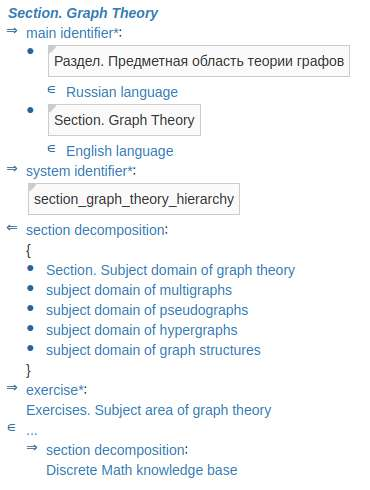
\includegraphics[width=8cm]{picture/1.jpg}
    \caption{\small{3D views of the zSurfH reference surface.}}
    \label{fig:example-a}
\end{figure}

\begin{figure}[H]
    \centering
    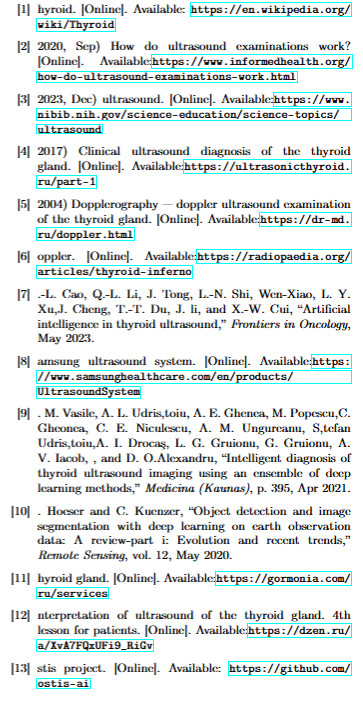
\includegraphics[width=8cm]{picture/2.jpg}
    \caption{\small{Contour map of the reference surface zSurfH}}
    \label{fig:example-b}
\end{figure}



of representative calculation results using the Wolfram Mathematica FindClusters function with different criteria of Criterion Function, we will explain the illustrations. The schemes in \autoref{fig:example-d} repeat the graphic layers from the maps above, they are useful for interpretation and explanation. The schema at the top details the reference, clearly marked sections of fragments-perturbations.

\fontsize{10}{14}
\selectfont 
\quad The schema below clearly shows areas where there is noreproduction of the standard, which is explained by
the lack of measurements. The contour map with data
points at the bottom is useful for understanding that in some areas the field cannot be restored to the standard



\begin{figure}[H]
    \centering
    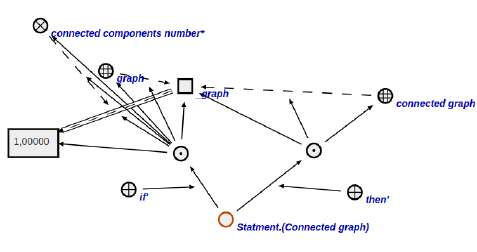
\includegraphics[width=8cm]{picture/3.jpg}
    \caption{\small{ A scheme of the measurement points of the levels, a map of the isolines of the reference and reconstructed surfaces.}}
    \label{fig:example-c}
\end{figure}

because there are no measurements. It is clear that in parts of the area where the digital field differs from the reference, classification / binding to a fragmentdisturbance is unlikely

\begin{figure}[H]
    \centering
    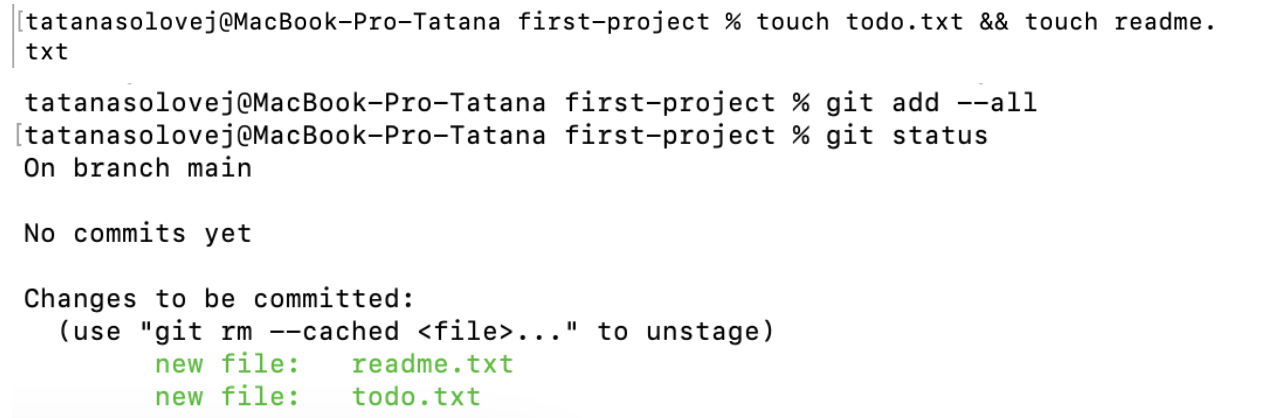
\includegraphics[width=8cm]{picture/4.jpg}
    \caption{\small{Schemas for understanding the differences between the processed data and the reference.}}
    \label{fig:example-d}
\end{figure}

\fontsize{10}{14}
\selectfont 
\quad \autoref{fig:example-f} shows the results of clustering by two parameters (rProfXY) in the upper part, and by three (rProfXYZ) at the bottom. The upper illustration shows the results of calculations with the settings of the KMeans method, as in [7]. Below is the current implementation for the same method; in both versions, the metric is "default", the number of clusters is 6.

\fontsize{10}{14}
\selectfont 
\quad The proposed clustering method for three parameters is clearly preferable to the method for two, in particular,in terms of localization of fragments 1, 4 and 5. The 

\begin{figure}[H]
    \centering
    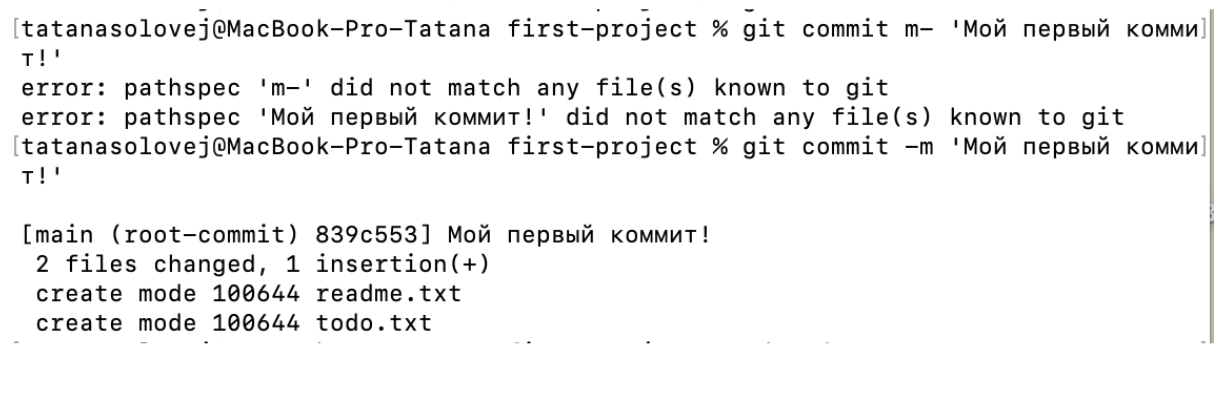
\includegraphics[width=8cm]{picture/5.jpg}
    \caption{\small{Schemas for understanding the differences between the processed data and the reference.}}
    \label{fig:example-f}
\end{figure}

results near fragments 2 and 3 are not indicative due to the discontinuous distribution on different sides of the horizontal dotted magenta line (projection onto the horizontal plane of the fragment section-perturbation 3
by the vertical plane).

\fontsize{10}{14}
\selectfont 
\quad
Such situations (gaps, offset) are not identified at all in conventional digital field restoration systems without special a priori additional conditions. Note that in the GeoBazaDannych, such conditions can be set interactively by correcting the initial information on the map[3].

\fontsize{10}{14}
\selectfont 
\quad
The figure shows the results of the variant when
the number of clusters is set to 6. Why. Determining
the number of clusters is one of the most important
segmentation problems. In a broader sense, this is the problem of initializing the algorithm. The results of the variants for the number of clusters from 4 to 9 were calculated and compared. According to the results of the comparison, the variant of 6 clusters seems preferable, and the explanation for this may probably be that the distribution is reproduced when there is a basic continuous
surface-a ribbon and 5 fragments-perturbations, i. e. 6 different shapes.

\fontsize{10}{14}
\selectfont
\section*{\textbf{A.The impact of the clustering method}}

\fontsize{10}{14}
\selectfont 
\quad
The variants of clustering results using different metho0s and metrics are illustrated in Figures 6 and 7, the names of the methods and metrics are written


\end{multicols}
\end{document}